% 中文初稿 v2；基于 results_time_aware_v3；使用 XeLaTeX 编译。
% 作者信息待填写；原始模板保留在 ../中文LaTeX模版/。
\documentclass[journal]{IEEEtran}
\usepackage{amsmath,amssymb,mathtools}
\usepackage{algorithm,algpseudocode}
\usepackage{comment}
\floatname{algorithm}{算法}
\usepackage{array,booktabs,graphicx,caption,cite,url,xcolor,hhline}
\usepackage[letterpaper]{geometry}
\geometry{tmargin=0.55in,bmargin=1.0in,lmargin=0.65in,rmargin=0.65in}
\setlength{\headheight}{48pt}
\setlength{\headsep}{14pt}
\usepackage{xeCJK}
\IfFontExistsTF{Noto Serif CJK SC}{\setCJKmainfont{Noto Serif CJK SC}}{%
  \IfFontExistsTF{FandolSong-Regular}{\setCJKmainfont{FandolSong-Regular}}{\setCJKmainfont{SimSun}}}
\IfFontExistsTF{Noto Sans CJK SC}{\setCJKsansfont{Noto Sans CJK SC}}{%
  \IfFontExistsTF{FandolHei-Regular}{\setCJKsansfont{FandolHei-Regular}}{\setCJKsansfont{Microsoft YaHei}}}
\IfFontExistsTF{Noto Sans Mono CJK SC}{\setCJKmonofont{Noto Sans Mono CJK SC}}{%
  \IfFontExistsTF{FandolFang-Regular}{\setCJKmonofont{FandolFang-Regular}}{\setCJKmonofont{SimSun}}}
\renewcommand{\abstractname}{\textcolor{violet}{\textbf{ABSTRACT / 摘要}}}
\newcommand{\flogo}{\IfFileExists{LOGO1.png}{
\includegraphics[height=40pt]{LOGO1.png}}{\textsf{S.H.I.T.}}}
\usepackage{fancyhdr}
\pagestyle{fancy}
\fancyhf{}
\lhead{\flogo}
\rhead{\IfFileExists{LOGO2.png}{
\includegraphics[height=40pt]{LOGO2.png}}{\textsf{研究初稿}}}
\renewcommand{\headrulewidth}{0pt}
\pagenumbering{gobble}
\setlength{\emergencystretch}{1em}
\newcommand{\clip}{\operatorname{clip}_{[0,100]}}
\newcommand{\pos}[1]{\left[#1\right]_+}
\makeatletter
\ifCLASSOPTIONjournal
\def\abstract{\@IEEEtweakunitybaselinestretch{1.15}%
\@IEEEabskeysecsize\noindent\abstractname---\relax
\fi\@IEEEgobbleleadPARNLSP}
\makeatother

\begin{document}
\title{\vspace*{0.5cm}\textcolor{violet}{今天去不去工位？\\基于强化学习的科研行为规划}\vspace*{0.5cm}}
\author{\textbf{陌玉菜菜子$^{1,*}$，小智$^{1}$}\\\vspace*{0.1cm}
\small $^{1}$ 东大村\\\vspace*{0.1cm}
$^{*}$ 通讯作者：陌玉菜菜子（e-mail: \texttt{mon4ter@mail.nwpu.edu.cn}）\\\vspace*{0.1cm}
本项目受S.H.*.T期刊“用 AI，解决真实问题”悬赏榜资助，具体悬赏内容为“身体、睡眠与健康管理”。\normalsize}
\twocolumn[{
\begin{@twocolumnfalse}
\let\newpage\relax\maketitle\thispagestyle{fancy}

\begin{abstract}
科研任务通常具有明确的交付期限，但人的精力与心态不能保持一致充足。本文将工科研究生的日常行为进行建模，研究在任务必须全部完成的条件下，能否减少以透支为代价的完成。本文提出的模型固定时间和任务量，同时考虑时段收益差异、夜间恢复、进度压力与随机导师检查。比较固定作息、睡懒觉、加班、延期、以及强化学习算法推导的作息情况。分别评价最终完成率、按时完成率与累积透支成本。在100个共同环境种子上，全部策略均完成任务，除延期方案外均按时交付。固定作息与三个强化学习训练种子的学习策略表现一致，平均透支成本为6.1838，较加班的49.2100降低约87.43\%。延期方案将透支成本进一步降至5.5051，但完成时间推迟一周，平均导师满意度由优化按时方案的93.32降至3.62。结果表明，在当前模型中，合理配置工作与恢复活动能够降低综合过程代价，提前交付和延期均存在状态与外部评价方面的取舍；学习策略尚未显示出超越优化固定日程的优势。本文属于未经现实数据校准的计算实验，其意义在于将任务完成与研究者的消耗分别评价，而非提供普遍适用的作息方案。

\\[0.8em]
\\
\noindent\textcolor{violet}{\textbf{INDEX TERMS / 关键词}} 科研行为规划；Q-learning；工作与恢复；有限延期；透支成本\\[0.8em]
\textcolor{violet}{\textbf{IMPACT STATEMENT / 影响声明}} 本文以可复现的仿真实验，探讨科研任务必须完成时如何降低过程代价，提示任务安排应同时关注交付要求、恢复机会与外部评价。实验参数未经现实数据校准，结果不构成健康建议或通用作息方案。希望科研计划在要求任务完成的同时，也为完成任务的人保留余量。
\vspace{0.4cm}
\end{abstract}
\end{@twocolumnfalse}
}]
\IEEEpeerreviewmaketitle

\section{INTRODUCTION / 引言}

研究生的科研工作不仅涉及知识与技术问题，也涉及日常行为的持续安排。阅读文献、编写程序、开展实验、分析结果与撰写论文需要投入时间，而吃饭、睡眠、休息和运动同样需要占据日程。对于具有明确截止日期的任务，研究者需要决定何时工作、何时恢复，以及是否接受一定程度的延期。这些选择看似只是“今天去哪里”，却会影响后续可用资源和任务推进方式。

与执行预先确定步骤的生产任务相比，科研工作的进展往往具有不确定性。一次实验可能需要重复，程序可能在运行结束后才暴露问题，原本预计用于整理结果的时间也可能转而用于排查错误。在这样的情境中，延长工作时间是一种容易实施的调整方式，但它是否能够形成更合适的长期安排，需要同时考虑任务进度和执行过程中的代价。研究计划可以通过修改日期获得延期，研究者的恢复过程则未必能通过修改表格完成。

科研任务的评价通常具有清晰的交付节点，例如阶段汇报、实验结果或论文提交。相比之下，完成任务期间的精力变化、情绪波动和恢复安排较难被同一张进度表描述。因此，“任务已经完成”与“任务以较低代价完成”应当作为两个不同的问题讨论。较早交付可能减少任务持续时间，也可能依赖缺少恢复的安排；适度延长执行时间可能降低工作密度，却也可能增加进度压力和外部评价代价。单独比较完成速度，无法充分表达这些取舍。

基于上述问题，本文提出一个具有明确约束的研究目标：
\textbf{任务必须完成时，能否减少以透支为代价的完成方式？}
这里的“透支”模型是表征精力亏空、焦虑及低状态代价的统称。本文关注在完成相同任务量的前提下，不同行为安排如何改变过程成本，同时分别报告最终完成率与按时完成率，避免以未完成任务换取较低成本。

\begin{figure}[t]
\centering
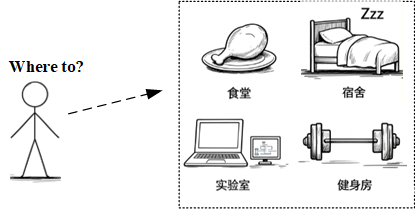
\includegraphics[width=0.4\textwidth]{where to.png}
\caption{抉择：今天去不去工位}
\label{fig:backgroundchoices}
\end{figure}

强化学习为这一问题提供了序贯决策的描述方式：一次行动不仅产生当前收益，也会改变下一时段的资源和选择条件。本文采用表格型Q-learning更新规则\cite{watkins1992}，让策略在仿真环境中通过行动及其反馈学习安排。但学习算法的引入并不意味着固定作息必然落后。一张合理的日程表本身就是有效的决策规则，因此本文同时保留简单循环和经过搜索的固定日程作为对照，以检验在线学习是否带来额外收益。

具体而言，本文将研究生的科研生活简化为实验室、宿舍和健身房三个动作，设置工作量、精力、心情、导师满意度与焦虑等状态，并引入时段收益差异、晚间自然恢复、随机导师检查和有限延期。任务目标期限为四周，最多允许延期一周。我们比较六类策略，并通过工作进度和状态轨迹解释其累计成本差异。学习策略采用固定日程示范初始化后继续在线Q-learning，因此其表现需要与示范日程直接比较，不能被解释为完全从零发现作息。

本文定位为一项以科研生活为题材的探索性计算实验。研究参数设定、策略比较、数据记录与结果解释遵循可核查、可复现的原则。模型参数由生活情境启发，由此得到的结果能够揭示当前规则下的行为机制和评价取舍，而不能直接确定现实中的最佳作息。

本文的主要工作是构建具有任务期限与恢复机制的科研行为环境，比较固定安排与示范辅助学习策略，并分析低成本完成、按时交付及外部评价之间的关系。第二章介绍环境与任务，第三章给出成本、奖励及策略设计，第四章报告实验结果，第五章讨论模型机制及现实启示，第六章总结研究结论。
\section{环境与任务}

\subsection{任务与状态}

每个回合模拟一项总量为48单位的科研任务，每天分上午、下午、晚上三个时段。目标期限为28天（84时段），最多延期7天，硬截止为35天（105时段），延期不改变任务量。

状态由剩余工作量$W$、精力$E$、心情$M$、导师满意度$S$和焦虑$A$构成，初值为
\begin{equation}
(W_0,E_0,M_0,S_0,A_0)=(48,100,60,60,0).
\end{equation}
$M,S,A$限制在$[0,100]$，$E$上限为100。工作量以0.1单位整数刻度存储，末次进度不超过剩余工作量。任务全部完成且未失败才记为成功；$E<0$、$A\ge100$或硬截止时仍未完成均记为失败。心情为0不直接终止回合，因此完成任务与维持状态需要分别评价。

\subsection{动作与恢复}

可选动作为实验室工作（$L$）、宿舍休息（$D$）和健身（$G$），直接收益见表~\ref{tab:actions}。所有参数均为未经现实数据校准的仿真假设。

\begin{table}[ht]
\begin{center}
\small
\resizebox{\columnwidth}{!}{%
\begin{tabular}{lrrrr}
\multicolumn{5}{c}{\textsc{动作与直接状态收益}} \\
\hhline{=====}
动作 & 工作量 & 精力 & 心情 & 焦虑\\
\hline
实验室 & $1/1.1/0.9$ & $-7$ & $-4$ & $+1$\\
宿舍 & $0$ & $8/6/12$ & $1/0/3$ & $-6$\\
健身房 & $0$ & $-2$ & $+7$ & $-8$\\
\hhline{=====}
\end{tabular}%
}
\end{center}
\caption{各动作的直接收益。斜线依次表示上午、下午、晚上；未分时段的数值在三个时段相同。}
\label{tab:actions}
\end{table}

若全天三个时段均工作，晚间额外扣除4点精力、6点心情，并增加3点焦虑。自然恢复仅在晚间动作、额外消耗及日末评价完成且未失败后结算：
\begin{equation}
R=\max\{2,8-\lfloor A/20\rfloor\}.
\end{equation}
晚间工作时恢复量改为$\max(2,R-2)$。上午或下午完成任务不获得夜间恢复；晚上完成仍须经过当晚结算，不能以完成任务跳过失败检查。

\subsection{进度压力与延期}

每周等概率生成0至3次导师检查，从周一至周五不重复抽取检查日，并在上午、下午中等概率选择检查时段。未来检查安排不向策略公开。检查时在实验室，$S$增加6；否则减少12。

令$t$为已执行时段数，相对28天目标的进度落后量为
\begin{equation}
\ell_t=\max\{0,48\min(t/84,1)-(48-W_t)\}.
\end{equation}
每日结束时，$M$和$S$每低于50、35、20、10中的一个阈值，分别增加1点焦虑，再叠加$\lfloor0.15\ell_t\rfloor$。每周末无落后时，$S$增加8；否则减少14，并增加$\lfloor2+\min(w,4)+0.3\ell_t\rfloor$点焦虑，其中$w$为周序号。第29至35天每日开始扣除2点心情，当日上午完成也不豁免。

各策略共用一步精力保护，排除预计会使精力为负的动作，并考虑全天工作额外消耗。规则策略遇到不可行动作时改为宿舍，学习策略在可行动作中选择。该保护不保证避免后续焦虑失败。

时段更新顺序见算法~\ref{alg:settlement}。夜间恢复位于失败检查之后，过程成本按完整时段结算后的状态计算，定义见式~\eqref{eq:cost}。

\begin{algorithm}[H]
\caption{单个时段的状态更新与结算}
\label{alg:settlement}
\footnotesize
\begin{algorithmic}[1]
\Require 当前状态、时段与可行动作
\Ensure 新状态、奖励与结束标记
\State 若为延期日上午，心情扣除2点
\State 执行动作与导师检查，更新状态
\State 检查精力耗尽或焦虑达到上限
\If{当前为晚上且未失败}
    \State 若全天工作，结算额外消耗；检查失败
    \If{未失败}
        \State 结算日末焦虑；若为周末，评价进度
        \State 检查失败
        \If{未失败}
            \State 结算自然恢复
        \EndIf
    \EndIf
\EndIf
\State 累计成本并计算奖励
\State 判定成功、失败或硬截止未完成
\end{algorithmic}
\end{algorithm}

\section{模型设计}

\subsection{观测与过程成本}

Q表采用离散观测
\begin{equation}
\begin{split}
o_t=\big(&t,10W_t,\lfloor E_t/10\rfloor,\lfloor M_t/5\rfloor,\\
&\lfloor S_t/20\rfloor,\lfloor A_t/10\rfloor,n_t^L\big),
\end{split}
\end{equation}
其中$n_t^L$为当天已执行的实验室动作数。绝对时间与剩余工作量保留精确刻度，其他变量分箱。由于未来导师检查不可见，且分箱损失部分状态信息，该观测并非完整环境状态，不能据此保证学习得到全局最优策略。

令$[x]_+=\max(0,x)$，每个时段结算后的成本定义为
\begin{equation}
\begin{split}
c_t={}&\frac{100-\max(0,E_t)}{100}+\frac{A_t}{100}\\
&+\frac{[30-M_t]_+}{30}+\frac{[25-E_t]_+}{25},
\end{split}
\label{eq:cost}
\end{equation}
分别表示精力亏空、焦虑、低心情和低精力。最后一项额外惩罚精力低于25的状态。累计透支成本为
\begin{equation}
C=\sum_{t=1}^{T}c_t,
\end{equation}
其中$T$为回合实际执行的时段数，晚间成本在自然恢复后采样。上述指标是仿真评价约定，不是健康量表；导师满意度不直接计入成本，但可通过焦虑间接影响成本。

本文分别报告最终完成率、按时完成率和累计成本。采用累计量意味着延期增加的时段也需计入代价，避免以日均成本下降掩盖执行时间延长。

\subsection{奖励与学习方法}

时段奖励为
\begin{equation}
\begin{split}
r_t={}&20\Delta P_t-c_t
+1000\mathbf{1}_{\mathrm{成功}}\\
&-500\mathbf{1}_{\mathrm{失败或硬截止未完成}},
\end{split}
\end{equation}
其中$\Delta P_t$为本时段完成的工作量，终止奖励仅在回合结束时给出。取折扣因子$\gamma=1$，成功完成48单位任务时有
\begin{equation}
\sum_{t=1}^{T}r_t=1960-C.
\end{equation}
因此，成功轨迹的回报排序与成本排序一致。奖励不另设按时完成奖金，28天目标通过进度压力与延期心情损失影响决策。有限失败惩罚不构成必然完成的保证，完成率仍须独立检验。

采用表格型Q-learning更新\cite{watkins1992}：
\begin{equation}
\begin{split}
Q(o_t,a_t)\leftarrow Q(o_t,a_t)+\alpha\big[
&r_t+\gamma V(o_{t+1})\\
&-Q(o_t,a_t)\big],
\end{split}
\end{equation}
非终止状态下，$V(o)$为可行动作中的最大Q值；终止状态下取0。学习率$\alpha=0.15$。每个训练种子先进行2000回合优化固定日程的示范更新，再进行10000回合$\epsilon$-greedy在线学习。在线探索率由0.1开始，每500回合乘0.8，最低为0.005；评估时关闭探索与更新，同值动作随机选择。

本文将该方法称为“示范初始化加在线Q-learning”。示范阶段按固定日程行动，在线及评估阶段由Q表选取动作。由于观测包含绝对时间，Q表能够记忆日程，复现示范不能解释为从零自主发现方案。

\subsection{对照策略与评估}

固定策略搜索枚举长度为3、6、9个时段的循环，先筛除硬期限内理论工作量不足的候选，再用环境种子41000初筛。按时与允许延期两类目标分别保留低成本前40个候选，在20个开发种子42000至42019上比较。按时方案进一步调整每日动作排列，保持每日动作数量不变。该搜索仅覆盖有限候选，不证明全局最优。

以三元组表示上午、下午、晚上的安排，六类对照为：
\begin{enumerate}
    \item 常规固定作息：每日$(L,L,D)$。
    \item 上午补觉：每日$(D,L,L)$。
    \item 简单三天循环：依次为$(L,L,D)$、$(L,L,D)$、$(G,L,G)$。
    \item 优化固定日程：在简单循环上，将第26天改为$(L,D,L)$，第28天上午休息、下午工作。
    \item 学习策略：以前述优化日程示范初始化，由Q表选择动作。
    \item 延期低成本循环：依次为$(D,L,G)$、$(D,L,G)$、$(D,L,L)$。
\end{enumerate}
任务结束后的计划动作不再执行，也不计入成本。

\begin{table*}[t]
\centering
\small
\setlength{\tabcolsep}{3pt}
\begin{tabular*}{\textwidth}{@{\extracolsep{\fill}}lrrrrrr@{}}
\multicolumn{7}{c}{\textsc{六种策略的总体评价结果}} \\
\hline\hline
策略 & 完成率 & 按时率 & 透支成本 & 完成时点
& 最终心情 & 导师满意度\\
\hline
常规固定作息（加班）
& 100\% & 100\% & 49.2100 & 第23天下午 & 0 & 99.18\\
上午补觉（睡懒觉）
& 100\% & 100\% & 58.4558 & 第24天晚上 & 0 & 65.60\\
简单三天循环
& 100\% & 100\% & 6.2638 & 第28天上午 & 56 & 95.22\\
优化固定日程
& 100\% & 100\% & 6.1838 & 第28天下午 & 54 & 93.32\\
Q-learning
& 100\% & 100\% & 6.1838 & 第28天下午 & 54 & 93.32\\
延期低成本循环(delay)
& 100\% & 0\% & 5.5051 & 第35天下午 & 58 & 3.62\\
\hline\hline
\end{tabular*}
\caption{各策略的任务完成情况与过程代价。固定策略各评价100回合，学习策略为三个训练种子各评价100回合，使用相同的100个环境种子。成本、最终心情和导师满意度为回合均值；完成时点在各策略的评价样本中一致。}
\label{tab:main}
\end{table*}

最终评估采用100个共同环境种子4000000至4000099，与开发种子分离。固定策略各评估100回合；学习策略使用训练种子42、43、44，分别在相同100个环境种子上评估。学习策略共计300次运行，但仅包含100种独立检查安排。组图展示一个共同环境样本的时序轨迹，汇总结果采用全部评估回合，避免将单条曲线解释为平均表现。

\section{实验结果}
\subsection{总体完成情况与评价范围}

本节比较常规固定作息、上午补觉、简单三天循环、优化固定日程、示范初始化加在线Q-learning以及延期低成本循环六种策略。固定策略各在100个共同环境种子上评价；RL使用三个训练种子，每个训练种子在相同的100个环境中评价。因此，RL共有300条评价轨迹，但不代表300个独立环境。

表~\ref{tab:main}报告评价样本的总体结果。六种策略均完成全部48单位任务，样本完成率为100\%。除延期低成本循环外，其余策略的按时完成率均为100\%。这些比例描述本次有限样本的表现，不构成任意环境下的完成保证。



图~\ref{fig:strategy_states}进一步展示同一环境中六种策略的动态轨迹。图中环境种子为4000000，RL训练种子为42；这些曲线用于说明执行过程，不是100个环境的统计平均。所有实际轨迹均在任务完成时停止，未继续模拟以获取额外恢复。

\begin{figure*}[t]
\centering
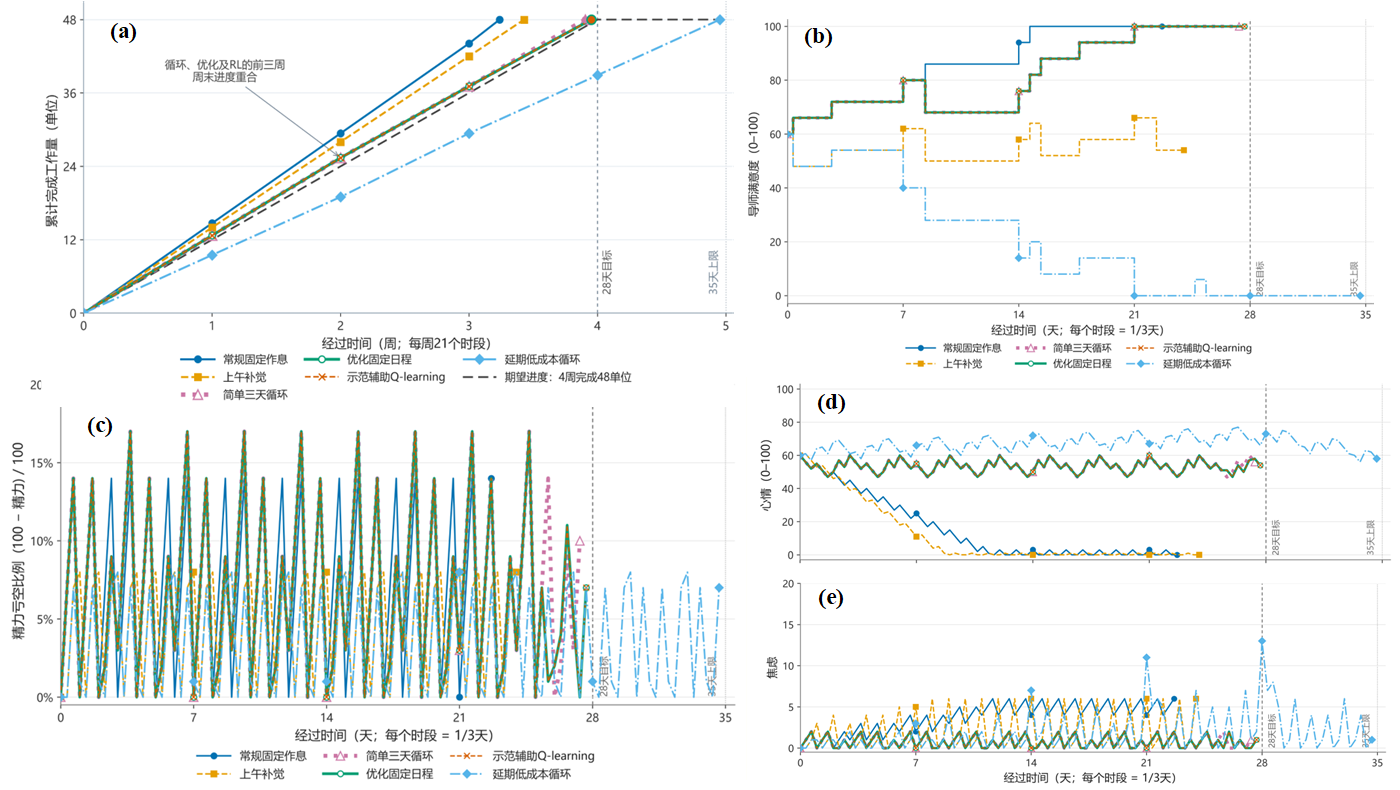
\includegraphics[width=\textwidth]{fig3v2.png}
\caption{六种策略在同一仿真环境中的进度与状态变化。
(a) 每周累计工作进度与期望进度；
(b) 导师满意度；
(c) 疲劳；
(d) 心情；
(e) 焦虑。}
\label{fig:strategy_states}
\end{figure*}

\subsection{任务进度与导师满意度}

图~\ref{fig:strategy_states}(a)显示，常规固定作息与上午补觉策略的工作进度持续领先于期望进度。两者在前三周末分别完成44.1和42.0单位工作，并于第23天下午和第24天晚上完成全部任务。简单三天循环、优化固定日程和RL的前三周末进度相同，分别为12.7、25.4和37.1单位，均略高于对应的12、24和36单位期望进度。简单循环于第28天上午完成；优化固定日程与RL于第28天下午完成。三者的工作安排更接近目标期限，而非尽可能提前结束。延期低成本循环的前三周末进度分别为9.5、19.0和29.4单位，第28天结束时完成38.9单位，仍有9.1单位未完成，最终于第35天下午结束。期望进度在第四周达到48单位后保持不变，延期期间不追加任务。因此，六种策略的差异主要体现在完成速度与执行代价，而非最终工作量。任务都交付了，但交付过程并不相同。



图~\ref{fig:strategy_states}(b)显示，导师满意度随随机检查和周末进度评价发生离散变化。常规固定作息在上午和下午持续工作，且进度领先，在示例中较早达到满意度上限。简单循环、优化固定日程与RL虽经历短暂下降，随后仍恢复至较高水平。上午补觉策略将部分工作安排在晚上，而导师检查仅发生在上午或下午。因此，即使任务进度领先，也可能因检查时不在实验室而受到扣分。其总体最终满意度均值为65.60，低于常规固定作息的99.18。延期策略同时面临进度落后与上午缺席，在示例中满意度后期多次降至0。其总体最终满意度均值仅为3.62，而优化固定日程为93.32。较低的过程成本因此伴随明显的外部评价代价。

\subsection{疲劳指标与恢复过程}

图~\ref{fig:strategy_states}(c)中的疲劳指标定义为
\[
F_t=\frac{100-\max(0,E_t)}{100},
\]
表示当前精力亏空比例，而非累计透支成本。曲线中的周期性升降对应工作消耗与休息恢复；晚间采样包含自然恢复，因此日内峰值与晚间低值可以同时存在。

在所示回合中，常规固定作息的最大精力亏空为14\%，上午补觉与延期循环为8\%，简单循环、优化固定日程和RL为17\%。这说明低总成本策略并不一定具有更低的瞬时疲劳峰值。

总体成本分解也呈现相同的取舍：优化固定日程的累计精力亏空成本为5.5400，高于常规固定作息的4.8300，但其总透支成本明显更低。因此，当前方案的主要改善不能解释为全面减少身体消耗，而应结合心情与焦虑共同判断。

\subsection{心情与焦虑变化}

图~\ref{fig:strategy_states}(d)显示，常规固定作息和上午补觉的心情持续下降，在示例中分别约于第12天和第9天首次降至0，此后在低值附近波动。两种策略虽然较早完成任务，却未能维持较好的模拟心情状态。

这一变化与直接动作收益一致：常规$(L,L,D)$作息每日心情净变化为$-5$，上午补觉$(D,L,L)$为$-7$。晚间工作增加后，上午较小的心情恢复收益不足以抵消两次工作消耗。

简单循环、优化固定日程和RL将恢复活动规律地安排在工作之间，示例中的心情主要保持在47至60之间。简单循环最终心情为56，优化固定日程与RL为54。延期循环的心情总体更高，但进入延期阶段后受到每日扣分影响，最终降至58。

图~\ref{fig:strategy_states}(e)进一步显示，简单循环、优化固定日程与RL的焦虑主要处于较低水平；常规固定作息和上午补觉在心情下降后出现更高的反复波动。延期策略虽维持了较高心情，仍因进度落后和导师满意度下降产生焦虑峰值，示例中的最大焦虑为13。由此可见，心情较高与压力较低并非同一指标。

\subsection{透支成本及延期权衡}

表~\ref{tab:components}分解了各策略的累计成本。常规固定作息的低心情成本为41.8000，占总成本约84.94\%；上午补觉的低心情成本进一步升至52.0000，是其总成本最高的主要原因。

\begin{table}[ht]
\centering
\small
\setlength{\tabcolsep}{3pt}
\begin{tabular*}{\columnwidth}{@{\extracolsep{\fill}}lrrrr@{}}
\multicolumn{5}{c}{\textsc{累计透支成本分解}} \\
\hline\hline
策略 & 精力亏空 & 焦虑 & 低心情 & 低精力\\
\hline
加班 & 4.8300 & 2.5800 & 41.8000 & 0\\
睡懒觉 & 3.7400 & 2.7158 & 52.0000 & 0\\
三天循环 & 5.6200 & 0.6438 & 0 & 0\\
优化／RL & 5.5400 & 0.6438 & 0 & 0\\
延期 & 3.5600 & 1.9451 & 0 & 0\\
\hline\hline
\end{tabular*}
\caption{各策略累计透支成本的四个分量，数值为评价回合均值。优化固定日程与学习策略的结果相同，合并展示。}
\label{tab:components}
\end{table}

优化固定日程消除了本次样本中的低心情成本，并降低焦虑成本，总成本由49.2100降至6.1838，相对常规固定作息降低约87.43\%。简单循环的成本为6.2638，仅比优化日程高0.0800，说明简单且规律的安排已经接近当前搜索所得的按时方案。

延期至第35天下午，可将成本进一步降低至5.5051，相对优化按时方案减少0.6787，约10.98\%。其中，精力亏空成本减少1.9800，焦虑成本增加1.3013。额外时间减轻了资源消耗，但没有消除进度与评价压力。

三个训练种子的RL均获得与优化固定日程相同的平均成本、完成时点、最终心情和动作分布。结合示例中重合的状态轨迹，当前结果支持学习策略保留了示范日程的表现，尚未显示出超越固定日程的收益。数万回合更新之后，算法对作息表表示了同意。

\subsection{延期心情惩罚的敏感性}

保持延期循环不变，将每日心情扣除量分别设为1、2和4，并在相同的100个环境种子上回放，结果见表~\ref{tab:sensitivity}。这一比较没有针对不同惩罚重新搜索或训练策略。

\begin{table}[ht]
\centering
\small
\setlength{\tabcolsep}{3pt}
\begin{tabular*}{\columnwidth}{@{\extracolsep{\fill}}rrrr@{}}
\multicolumn{4}{c}{\textsc{延期心情惩罚的敏感性比较}} \\
\hline\hline
每日心情扣除 & 完成率 & 平均成本 & 最终心情\\
\hline
1 & 100\% & 5.5051 & 65\\
2 & 100\% & 5.5051 & 58\\
4 & 100\% & 5.5051 & 44\\
\hline\hline
\end{tabular*}
\caption{同一延期日程在不同心情惩罚下的回放结果，未重新搜索或训练策略。各设置使用相同的100个环境种子，均于第35天下午完成，按时率均为0；成本与最终心情为回合均值。}
\label{tab:sensitivity}
\end{table}

惩罚增大使最终心情下降，但平均成本保持不变。回放中，这些心情差异未改变低心情成本及相关焦虑阈值的触发情况，其他成本分量也保持相同。因此，该结果说明当前分段成本对部分心情变化不敏感，不能解释为延期惩罚没有生效，也不能据此断言重新优化后的策略仍然相同。
\section{分析与讨论}

\subsection{加班}

常规固定作息在第23天下午完成任务，却具有较高的累积透支成本；优化固定日程在第28天下午完成，成本明显降低。两者的差异说明，在本模型中，更早交付与更低过程代价并不一致。常规作息虽然缩短了任务持续时间，但连续工作造成的心情损失累积较快，提前结束不足以抵消此前的代价。

这一现象对应现实中的科研计划可以同时考察交付时间与执行状态。例如，连续赶工是否影响后续任务，提前交付是否以取消全部恢复活动为条件，以及任务结束后是否仍能维持正常生活。本文没有模拟后续任务，不能量化这些影响，但可以指出仅看完成日期的局限：一张计划表可以显示全部提前，执行计划的人却可能已经进入待机状态。另一方面，低成本也不等于身体负担全面下降。优化固定日程的累积精力亏空高于常规作息，综合成本优势主要来自避免低心情状态。因此，结果更准确的含义是改变了代价的构成，而不是消除了代价。现实中的计划评价也需要查看具体指标，避免把一个较好的总分理解为所有方面都得到了改善。综合评分允许不同项目相互补偿，研究者本人未必愿意接受这种调剂。

\subsection{睡懒觉}

上午补觉方案的成本高于常规固定作息，不能据此推断上午休息在现实中无效。该方案将工作安排为下午和晚上；在当前设定下，上午休息的心情收益仅为1，低于晚上休息的3，晚间工作量也低于下午，并减少自然恢复。因此，较高成本来自整套日程与环境规则的共同作用，而非“补觉”这一动作本身。

这为现实安排提供了一个可检验的思路：改变一段时间的用途时，应同时检查被移动的工作去了哪里。上午留给休息，如果晚上因此承担更多工作，实际效果取决于个人状态、工作性质和恢复条件，不能只计算上午增加了多少空闲。把闹钟推迟两小时，并不自动意味着任务也会体谅地少做两小时。

简单三天循环与优化固定日程则通过引入健身和调整工作时段，避免了长期低心情。在模型中，健身虽然消耗精力，却补充心情并降低焦虑，因而能够改善后续轨迹。这提示科研计划中的恢复活动不必只有一种形式，也不必等到所有工作结束后才安排。但本文未验证真实运动效果，更不能规定统一的运动频率。这里值得借鉴的是为恢复预留位置：如果计划中的每个空格都默认属于工作，那么休息只能以临时故障的形式出现。

\subsection{延期}

延期方案的平均成本较优化按时方案降低约10.98\%，但完成时点推迟至第35天下午，平均导师满意度由93.32降至3.62。较长的执行时间允许更稀疏的工作安排，却同时增加进度落后和外部评价压力。因此，该方案只能称为当前成本定义下的低成本候选，不能据此认定为更好的整体选择。

这一取舍在现实任务管理中具有直接的讨论价值。延期是否合理，需要结合交付依赖、合作安排和新增时间的实际用途判断。若新增时间主要用于恢复与处理不确定性，可能具有价值；若延期同时伴随任务扩张，则未必能够降低负荷。申请多一周时间与获得多一周可支配时间，是两个需要分别核实的事实。前者可以通过修改日期完成，后者往往还需要抵抗“既然时间充裕，不如再加一个实验”。

导师满意度的下降还暴露了评价函数的范围限制。该变量未直接计入透支成本，只通过焦虑间接产生影响，因此低成本方案可以伴随很差的外部评价。现实中的沟通、合作与信誉也难以被一个个人状态指标覆盖。模型可以宣布成本下降，导师则可能要求解释为什么人也下降到了检查视野之外。

\subsection{心态}

将延期每日心情扣减由2改为1或4，并重放同一延期日程后，累积成本仍为5.5051，而最终心情分别为65、58和44。这一结果表明，在所测试样本与日程下，改变扣减幅度没有改变成本；它并不证明延期影响可以忽略，也不代表重新训练后仍会选择相同方案。

其原因在于成本函数只对心情低于30的部分施加直接惩罚，日末焦虑又采用分段阈值。心理状态发生变化时，如果尚未产生影响成本的差异，汇总数值便可能保持不变。换言之，指标没有变化，可能是状态确实稳定，也可能是尺子的刻度还不够细。

这一限制对应现实评价中的常见问题：没有触发异常标准，并不等于没有受到影响。“还没到需要处理的程度”可以描述阈值位置，却不能替代对状态变化的观察。本实验中的研究者可以从心情65降到44，而总成本仍表示一切如常；现实中的研究者未必愿意配合这种统计口径。评价任务安排时，因此有必要同时查看累积指标、最低状态和终局状态，而非只保留一个便于排名的数字。

\subsection{算法的贡献与现实使用边界}

三个训练种子的学习策略均复现优化固定日程，当前结果支持其保留示范方案的能力，没有显示出优于固定日程的证据。由于训练包含示范初始化，观测又保留绝对时间，Q表能够记忆与特定日期对应的动作。因此，本实验不能被解释为算法从零发现了科研生活的最优规律。

这一结果也有实际启发：改进计划未必需要先引入复杂工具。可以先用简单记录区分工作时间与有效进度，观察哪些连续安排容易造成状态下降，再比较少量可执行的替代方案。若一张固定日程已能满足需要，增加算法复杂度应有明确理由。本次Q-learning经过数万回合更新后认可了既有日程，至少说明它没有因为自己使用了强化学习，就坚持否认作息表的学术地位。

上述启发仍受模型边界约束。真实科研工作具有难度差异、返工、协作和突发事件，不能稳定地按时段兑换工作量；人的精力与心情也未必服从固定增减规则。更合适的现实使用方式，是将本文视为比较任务安排的思考工具：明确必须完成的工作，给恢复活动留出位置，并检查延期与赶工分别转移了哪些代价。

\section{总结}

本文围绕“任务必须完成时，能否减少以透支为代价的完成方式”构建科研行为仿真环境，在相同任务量、目标期限和检查样本下比较六类策略。所评估样本中，各策略均完成全部任务，但按时率与过程代价存在明显差异。优化固定日程与示范初始化加在线Q-learning均在第28天下午完成，平均透支成本较常规固定作息降低约87.43\%；延期方案的成本进一步降低约10.98\%，但失去按时交付，并伴随导师满意度显著下降。

上述结果表示，科研计划除了回答“什么时候做完”，还可以回答“以什么状态做完”。提前交付有其价值，但若依赖持续压缩恢复时间，其代价就需要一并评估。工作时间、完成进度与个人状态应分别记录，不能仅凭在工位停留的时长判断计划是否有效。研究者按时出现在实验室，能够证明门禁系统运行正常，尚不足以证明研究工作同样正常。

恢复活动也可以作为计划的组成部分，而非完成全部工作后的剩余安排。本实验中的低成本方案通过工作、休息与健身的配置维持状态，但并未使所有成本分项同时下降。因此，现实中的安排仍需根据个人情况与任务性质调整，不能把模拟日程直接当作生活处方。休息值得预留，也不必每次都提交一份关于次日生产率的论证；否则，床只是增加了卧姿功能的工位。

延期则需要同时考虑个人负荷与外部约束。它可能提供调整节奏的空间，也可能增加沟通、合作和后续交付的压力。新增时间是否有用，取决于其用途是否明确，以及任务是否随之扩张。若每次延期都附赠一个新实验，截止日期虽然向后移动，研究者与它的距离可能并没有改变。

本文采用人为参数和简化状态，未校准真实健康效果，也未覆盖科研任务的复杂性，结果仅适用于当前仿真条件。其价值在于以可复现的实验提醒我们：任务完成度与研究者的消耗程度，是两项需要同时讨论的结果。我们以严谨的手段进行娱乐，也希望留下一个认真可用的问题：当论文、代码和实验都被要求完成时，能否为完成它们的人保留一点余量？项目需要耗材，而研究者不应是耗材。

\section*{致谢}
本项目受S.H.*.T期刊“用 AI，解决真实问题”悬赏榜资助，具体悬赏内容为“身体、睡眠与健康管理”。


感谢在实验讨论中持续校正时段收益、延期规则与结果解释的参与者。作者在代码检查、实验整理及撰写过程中使用了AI辅助工具。本研究为计算机仿真实验，未开展人体试验或问卷调查。

\begin{thebibliography}{1}
\bibitem{watkins1992}
C. J. C. H. Watkins and P. Dayan, ``Q-learning,'' \textit{Machine Learning}, vol. 8, pp. 279--292, 1992. doi: 10.1007/BF00992698.
\end{thebibliography}
\end{document}




